%part2a.tex
\subsection*{a. Stability of the solutions of an ODE-system of LCC-type}
The purpose of this section is to investigate the stability of an ODE while a parameter changes continuously.

The given third-order equation is the following : 
\begin{eqnarray*}
y'''+3y''+2y'+Ky =& 0 \\
y(0) =& 1\\
y'(0)=&1\\
y''(0)=&1
\end{eqnarray*}

It is possible to rewrite this as a system of ODE's, introducing new variables.
\begin{eqnarray*}
\textbf{u'}  = \left( \begin{array}{c}
y' \\ 
y'' \\ 
y'''
\end{array} \right) =& \left( \begin{array}{ccc}
0 & 1 & 0 \\ 
0 & 0 & 1 \\ 
-K & -2 & -3
\end{array}  \right) \left( \begin{array}{c}
y \\ 
y'\\ 
y''
\end{array} \right) = \textbf{Au} 
\end{eqnarray*}
The initial conditions are rewritten by :
\begin{eqnarray*}
\textbf{u(0)} =& \left( \begin{array}{c}
y(0) \\ 
y'(0)\\ 
y''(0)
\end{array} \right) = \left( \begin{array}{c}
1\\ 
1\\ 
1
\end{array} \right) 
\end{eqnarray*}

The solutions, computed analytically for different values of K, are given in figure \ref{result21}. The Matlab code is given at the end of this section. It is possbile to see that for the first three values of K, the maximal amplitude of the blue curve (that is the function $y$) tends to decrease. This being an LCC system, we know that a perturbation will follow the same ODE so we can conclude that the system is stable for those values of K. On the other hand, for the last value ($K=8$), this amplitude increases. Hence, the system is not stable for $K=8$. By continuity, that means that the system becomes unstable for a value of K between $4$ and $8$. Because we know nothing else, the best estimation that we can give right now is that this value is $K=6$.\\

\begin{figure}
\begin{center}
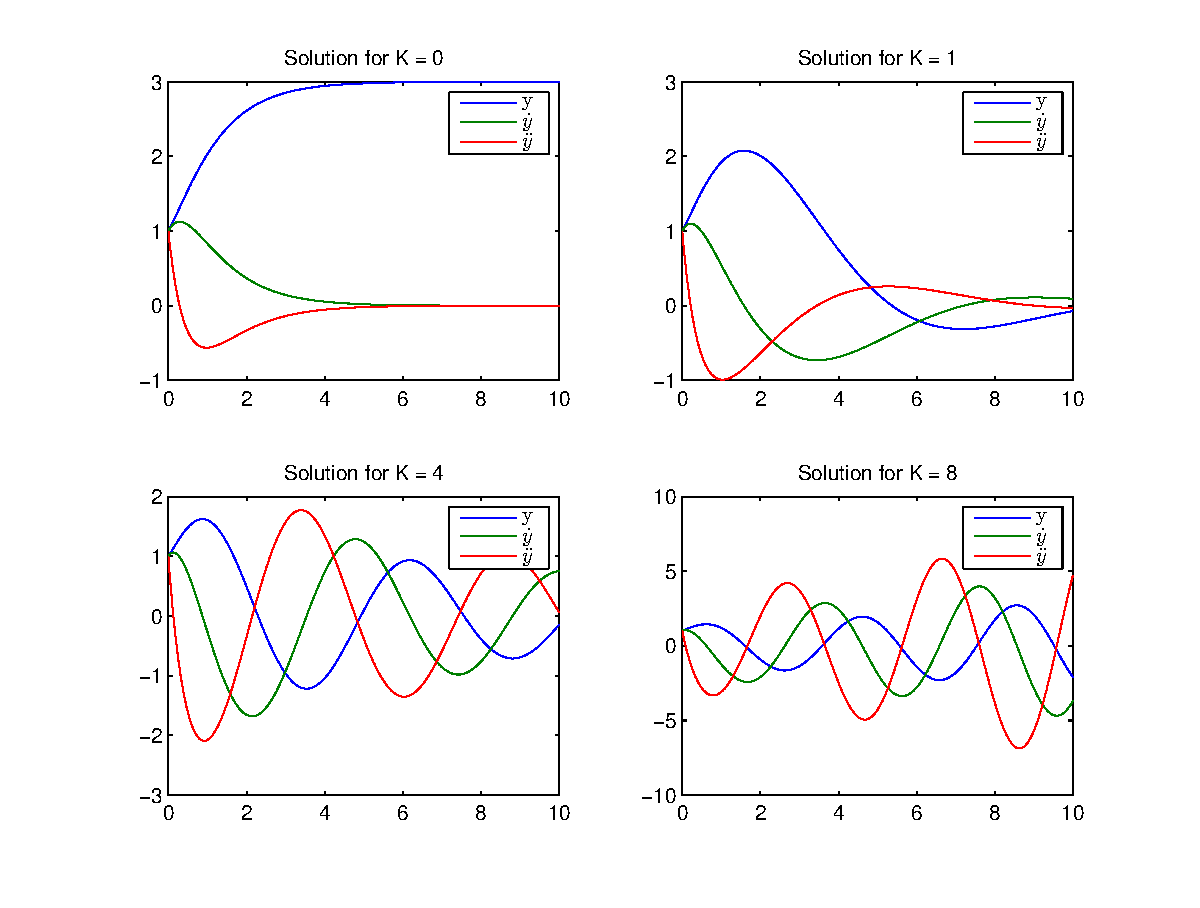
\includegraphics[scale=0.5]{result21.eps}
\caption{Solutions of the system in part 2a for various values of K}
\label{result21}
\end{center}
\end{figure}

We then drew a root locus to see how the system would evolve if K varies continuously. 


%Ce truc insere mon code MATLAB (nice!) 
\lstinputlisting{LAB1_21.m}